\renewcommand{\baselinestretch}{1.2} 
\chapter{Bài 13. Chuyển động của vật trong chất lưu}
\begin{center}
	\textit{(3 tiết)}
\end{center}
\begin{center}
	\textbf{(TIẾT 1: ÁP SUẤT THỦY TĨNH)}
\end{center}
\section{MỤC TIÊU DẠY HỌC}
\begin{center}
	\begin{longtable}{|M{2.5cm}|L{12.5cm}|M{2cm}|}
		\hline
		\thead{Biểu hiện\\ năng lực} & \thead{Mục tiêu} & \thead{STT}\\
		\hline
		\multicolumn{3}{|c|}{\textbf{ Năng lực vật lí}}\\
		\hline
		1.1 & Nêu được khối lượng riêng của một chất là khối lượng của một đơn vị thể tích của chất đó. & 1\\
		\hline
		1.1 & Nêu được áp suất được xác định bằng độ lớn áp lực trên một đơn vị diện tích bị ép $p=\dfrac{F}{S}$. & 2\\
		\hline
		1.2 & Thành lập được phương trình $\Delta p=\rho g\Delta h$. & 3\\
		\hline
		3.1& Vận dụng được phương trình $\Delta p=\rho g\Delta h$ trong một số trường hợp đơn giản. & 4\\
		\hline
		\multicolumn{3}{|c|}{\textbf{Năng lực chung}}\\
		\hline
		TC - TH& Tích cực thực hiện các nhiệm vụ GV đặt ra cho các nhóm, tích cực suy luận để đưa ra câu trả lời trong quá trình GV định hướng nội dung học tập	&5 \\
		\hline
	\end{longtable}
\end{center}
\section{THIẾT BỊ DẠY HỌC VÀ HỌC LIỆU}
\begin{itemize}
	\item Tivi/máy chiếu;
	\item SGK;
\end{itemize}
\section{TIẾN TRÌNH DẠY HỌC}
\subsection{TIẾN TRÌNH}\newpage
\begin{center}
	\begin{longtable}{|L{2.75cm}|C{1.25cm}|L{5cm}|L{3.5cm}|L{4cm}|}
		\hline
		\thead{Tiến trình} & \thead{Mục\\tiêu} & \thead{Nội dung dạy học \\trọng tâm} & \thead{PP,\\ KTDH} & \thead{Phương pháp \\đánh giá}\\
		\hline
		\textbf{Hoạt động 1: Sửa bài tập phát triển tư duy}& 5 & Sửa bài tập phát triển tư duy về chuyển động ném ngang mà GV đã giao về nhà cho HS. & PPDH: Đàm thoại & GV đánh giá dựa trên câu trả lời của HS.\newline
		PP đánh giá: quan sát, nghe.\\
		\hline
		\textbf{Hoạt động 2: Ôn tập khái niệm áp suất} & 1, 2 & Ôn tập khái niệm áp suất HS được học trong chương trình KHTN. & PPDH: Đàm thoại &  GV đánh giá dựa trên câu trả lời của HS.\newline
		PP đánh giá: quan sát, nghe.\\
		\hline
		\textbf{Hoạt động 3: Thành lập phương trình $\Delta p=\rho g\Delta h$} & 3 & Thành lập phương trình xác định độ chênh lệch áp suất giữa hai điểm trong lòng chất lỏng $\Delta p=\rho g\Delta h$. & PPDH: Thuyết trình &GV đánh giá dựa trên câu trả lời của HS.\newline
		PP đánh giá: quan sát, nghe.\\
		\hline
		\textbf{Hoạt động 4: Vận dụng phương trình $\Delta p=\rho g\Delta h$} & 4, 5 & Vận dụng phương trình xác định độ chênh lệch áp suất giữa hai điểm trong lòng chất lỏng $\Delta p=\rho g\Delta h$ trong một số bài tập đơn giản. & PPDH: Thuyết trình\newline KTDH: Tia chớp &GV đánh giá dựa trên câu trả lời của HS.\newline
		PP đánh giá: quan sát, nghe.\\
		\hline
	\end{longtable}
\end{center}
\hoatdong{Sửa bài tập phát triển tư duy}
{HS vận dụng được biểu thức xác định tầm xa của vật chuyển động ném ngang.
}
{Kết quả trả lời của HS cho câu hỏi GV đã giao.\\
	
}
{\textit{\underline{* GV chuyển giao nhiệm vụ học tập}}\\
	GV giao trước bài tập về nhà cho HS ở cuối tiết học trước (Câu 21, Câu 22 - Đề luyện tập Chuyển động ném ngang).\\
	\setcounter{ex}{20}
	% ======================================================================
	\begin{ex}
		\immini{Trong hình bên, bốn lá sen nhô lên khỏi mặt nước và một con ếch đang ở ngồi trên bờ hồ. Cho rằng độ cao của bờ hồ và lá sen so với mặt nước lần lượt là $H=6h$, $h_a=h_b=4h$, $h_c=h_d=h$. Ếch và tâm của hai lá sen a, b cùng nằm trên một mặt phẳng thẳng đứng. Giao điểm của thân bốn lá sen với mặt nước là bốn đỉnh của một hình vuông song song với bờ sông và có chiều dài cạnh bằng $\ell$. Khoảng cách theo phương ngang giữa lá sen a và bờ hồ cũng là $\ell$. Xem con ếch chuyển động như vật ném ngang với gia tốc trọng trường $g$.}
		{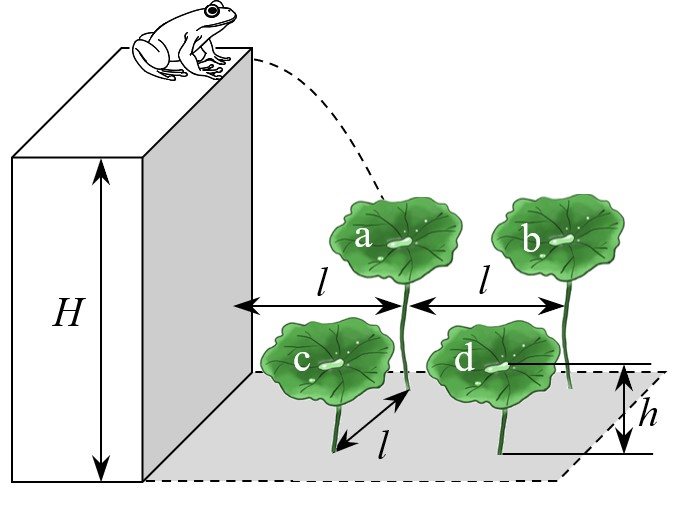
\includegraphics[scale=0.6]{../figs/G10-BTNEMNGANG2-5}}
		\begin{enumerate}[label=\alph*)]
			\item Sau một cú nhảy, con ếch đã đậu thành công trên lá sen a. Tìm tốc độ ban đầu của con ếch.
			\item Tốc độ nhảy ban đầu của con ếch ứng với sự rơi trên lá sen nào là nhỏ nhất? Giải thích một cách tường minh.
		\end{enumerate}
		\loigiai{\begin{enumerate}[label=\alph*)]
				\item $v_{0a}=\ell\sqrt{\dfrac{g}{4h}}$.
				\item $v_{0b}=\ell\sqrt{\dfrac{g}{h}}$; $v_{0c}=\ell\sqrt{\dfrac{g}{5h}}$; $v_{0d}=\ell\sqrt{\dfrac{g}{2h}}$.\\
				Tốc độ ban đầu ứng với sự nhảy trên lá sen c là nhỏ nhất.
		\end{enumerate}}
	\end{ex}
	\textit{\underline{* HS thực hiện nhiệm vụ học tập}}\\
	HS làm bài tập tại nhà.\\
	\textit{\underline{* HS báo cáo kết quả nhiệm vụ học tập}}\\
	GV mời HS lên bảng giải bài tập.\\
	Cả lớp chú ý theo dõi, đặt câu hỏi.\\
	GV chỉnh lí, hợp thức hóa kiến thức.
}
\hoatdong{Ôn tập khái niệm áp suất}
{HS nêu được áp suất được xác định bằng độ lớn áp lực trên một đơn vị diện tích bị ép $p=\dfrac{F}{S}$.
}
{Câu trả lời của HS cho các câu hỏi gợi mở của GV}
{\textit{\underline{* GV chuyển giao nhiệm vụ học tập}}\\
	GV đặt câu hỏi gợi mở vấn đề.\\
	Dùng hai ngón tay để bóp vào hai đầu của ghim giấy như hình minh họa. Ngón tay nào sẽ dễ bị tổn thương hơn? Vì sao?
	\begin{center}
		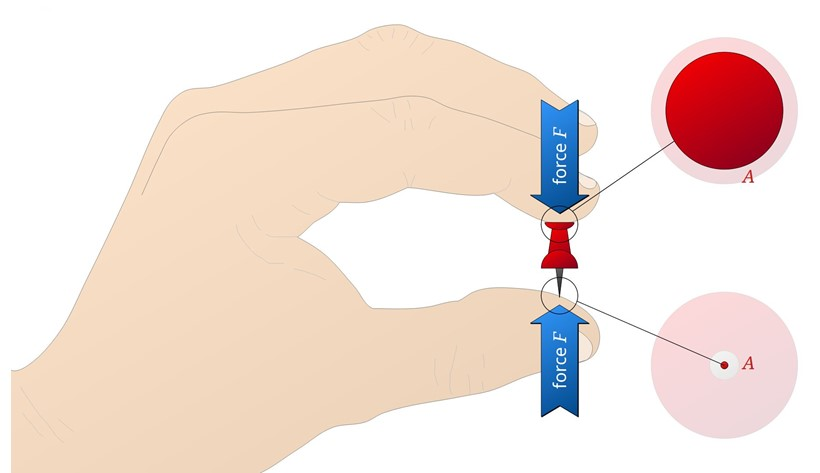
\includegraphics[scale=0.4]{../figs/G10-BAI13-1}
	\end{center}
	GV yêu cầu HS nhắc lại biểu thức xác định áp suất đã được học trong chương trình KHTN.\\
	GV yêu cầu HS kể tên 1 số đơn vị đo áp suất đã biết.\\
	\textit{\underline{* HS thực hiện nhiệm vụ học tập}}\\
	HS tích cực lắng nghe, suy nghĩ.\\
	\textit{\underline{* HS báo cáo kết quả nhiệm vụ học tập}}\\
	HS tích cực trả lời câu hỏi gợi mở của GV.\\
	HS chú ý theo dõi, đặt câu hỏi.\\
	GV chỉnh lí, hợp thức hóa kiến thức.

}
\hoatdong{Thành lập phương trình $\Delta p=\rho g\Delta h$}
{Dưới sự gợi ý của GV, HS thiết lập được phương trình $\Delta p=\rho g\Delta h$}
{Câu trả lời của HS cho các câu hỏi gợi mở của GV.
	\begin{enumerate}[label=\bfseries Bước \arabic*., leftmargin=2cm]
		\item Xét khối chất lỏng dạng khối lập phương trong lòng chất lỏng đang đứng yên. Khối chất lỏng này chịu tác dụng của các lực nào?\\
		\textit{Câu trả lời dự kiến:} Áp lực do chất lỏng gây ra trên 6 mặt của khối lập phương và trọng lực của khối nước.
		\item Điều kiện để một vật đứng yên là gì?\\
		\textit{Câu trả lời dự kiến:} Tổng hợp lực tác dụng lên vật bằng không.
		\item Xét điều kiện cân bằng của khối chất lỏng trên phương ngang và phương thẳng đứng để suy ra mối quan hệ về áp suất chất lỏng gây ra tại điểm 3-4 và 1-2?
		\begin{center}
			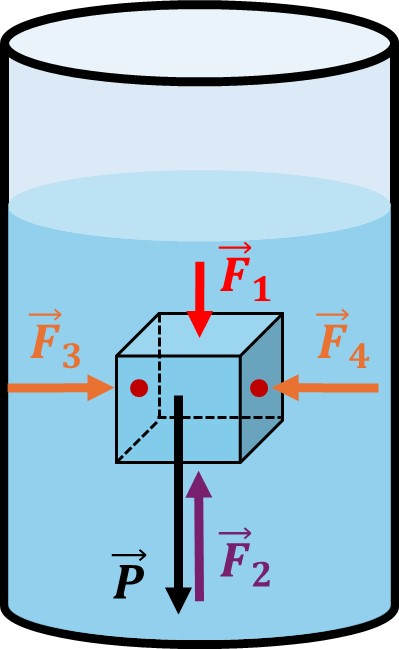
\includegraphics[scale=0.4]{{../figs/G10-BAI13-3}}
		\end{center}
		\textit{Câu trả lời dự kiến:}\\
		Trên phương ngang: $F_3=F_4\Rightarrow p_3=p_4$; $F_5=F_6\Rightarrow p_5=p_6$.\\
		Trên phương thẳng đứng:
		$F_2-F_1=P\Leftrightarrow \left(p_2-p_1\right)S=\rho gV\Rightarrow p_2-p_1=\rho g\Delta h$.
		\item Áp suất tại mặt thoáng chất lỏng bằng áp suất khí quyển $p_0$. Em hãy rút ra biểu thức xác định áp suất tại điểm trong lòng chất lỏng và cách mặt thoáng đoạn $h$.\\
		$$p=p_0+\rho gh.$$
	\end{enumerate}
}
{\textit{\underline{* GV chuyển giao nhiệm vụ học tập}}\\
	GV giới thiệu cho HS: Chất lỏng có xu hướng nén lên mọi vật nhấn chìm trong nó những lực theo mọi phương và vuông góc với bề mặt của vật.\\
	GV gợi mở cho HS thiết lập biểu thức xác định độ chênh lệch áp suất giữa hai điểm trong lòng chất lỏng.\\
	\vspace{-1cm}
	\begin{enumerate}[label=\bfseries Bước \arabic*., leftmargin=2cm]
		\item Xét khối chất lỏng dạng khối lập phương trong lòng chất lỏng đang đứng yên. Khối chất lỏng này chịu tác dụng của các lực nào?
		\begin{center}
			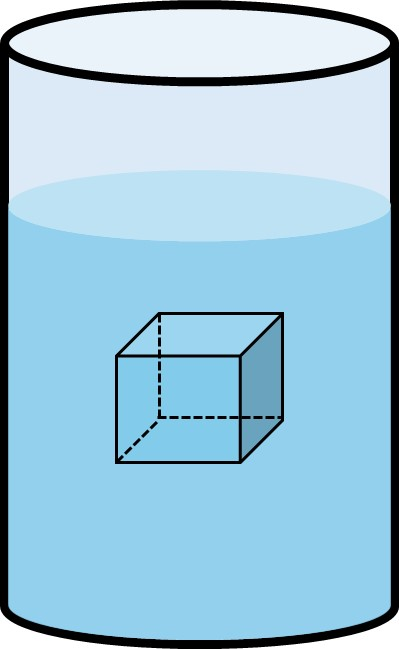
\includegraphics[scale=0.4]{../figs/G10-BAI13-2}
		\end{center}
		\item Điều kiện để một vật đứng yên là gì?
		\item Xét điều kiện cân bằng của khối chất lỏng trên phương ngang và phương thẳng đứng để suy ra mối quan hệ về áp suất chất lỏng gây ra tại điểm 3-4 và 1-2?
		\begin{center}
			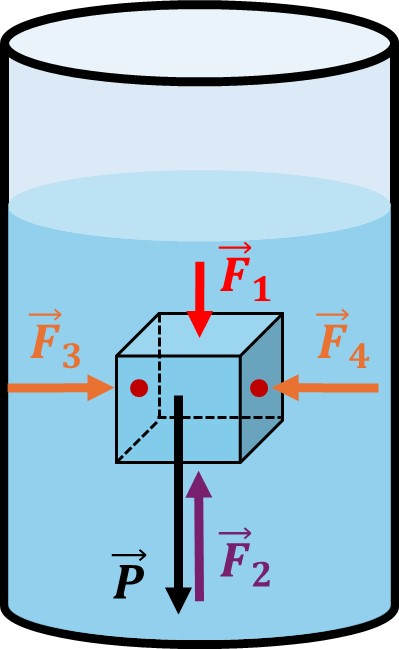
\includegraphics[scale=0.4]{{../figs/G10-BAI13-3}}
		\end{center}
		\item Áp suất tại mặt thoáng chất lỏng bằng áp suất khí quyển $p_0$. Em hãy rút ra biểu thức xác định áp suất tại điểm trong lòng chất lỏng và cách mặt thoáng đoạn $h$.
	\end{enumerate}
	 \textit{\underline{* HS thực hiện nhiệm vụ học tập}}\\
	 HS tích cực lắng nghe, suy nghĩ.\\
	 \textit{\underline{* HS báo cáo kết quả nhiệm vụ học tập}}\\
	 HS tích cực trả lời câu hỏi gợi mở của GV.\\
	 HS chú ý theo dõi, đặt câu hỏi.\\
	 GV chỉnh lí, hợp thức hóa kiến thức.

}
\hoatdong{Vận dụng phương trình $\Delta p=\rho g\Delta h$}
{HS vận dụng được phương trình $\Delta p=\rho g\Delta h$ trong một số trường hợp đơn giản.
}
{Phần trình bày bài giải ví dụ của HS.
}
{\textit{\underline{* GV chuyển giao nhiệm vụ học tập}}\\
	GV lần lượt giao bài tập ví dụ cho HS và yêu cầu HS làm nhanh nhất sẽ lên bảng trình bày bài giải. HS trình bày bài giải đúng sẽ nhận được 1 điểm cộng.\\
\textit{\underline{* HS thực hiện nhiệm vụ học tập}}\\
HS giải bài tập cá nhân.\\
GV quan sát, hỗ trợ các HS gặp khó khăn.\\
\textit{\underline{* HS báo cáo kết quả thực hiện nhiệm vụ học tập}}\\
GV mời HS hoàn thành nhanh nhất lên bảng làm bài.\\
Các HS còn lại nhận xét, góp ý.\\
GV chỉnh lí, hợp thức hóa kiến thức.
}
\section{HỒ SƠ DẠY HỌC}
\subsection{NỘI DUNG DẠY HỌC}
\begin{enumerate}[label=\bfseries\Roman*.]
	\item \textbf{Áp suất}\\
	Áp suất có giá trị bằng áp lực trên một đơn vị diện tích
	$$p=\dfrac{F}{S}.$$
	Trong đó:
	\begin{itemize}
		\item $F$: áp lực $\left(\si{\newton}\right)$;
		\item $S$: diện tích $\left(\si{\meter^2}\right)$.
	\end{itemize}
	Áp suất chuẩn của khí quyển $p_0=\SI{1}{atm}=\SI{1.013E5}{\pascal}$.\\
	Một số đơn vị khác của áp suất:\\
	$\SI{1}{\pascal}=\SI{1}{\newton/\meter^2}$\\
	$\SI{1}{Torr}=\SI{1}{\milli\meter Hg}=\SI{133.3}{\pascal}$\\
	$\SI{1}{atm}=\SI{760}{\milli\meter Hg}$\\
	$\SI{1}{at}=\SI{0.96784}{atm}$\\
	$\SI{1}{bar}=\SI{0.98692}{atm}$.
	\item \textbf{Áp suất thủy tĩnh}\\
	Chất lỏng có xu hướng nén lên mọi vật nhấn chìm trong nó những lực theo mọi phương và vuông góc với bề mặt của vật.\\
	Trên cùng một mặt nằm ngang trong lòng chất lỏng, áp suất là như nhau tại tất cả các điểm.\\
	\textbf{Độ chênh lệch áp suất:}
	$$\Delta p=\rho g\Delta h.$$
	Trong đó:
	\begin{itemize}
		\item $\rho$: khối lượng riêng của chất lỏng $\left(\si{\kilogram/\meter^3}\right)$;
		\item $g$: gia tốc trọng trường $\left(\si{\meter/\second^2}\right)$;
		\item $\Delta h$: độ chênh lệch độ cao giữa hai điểm trong chất lỏng $\left(\si{\meter}\right)$.
	\end{itemize}
	\textbf{Áp suất thủy tĩnh ở độ sâu $h$}
	$$p=p_0+\rho gh.$$
	Trong đó $p_0$ là áp suất khí quyển ở bề mặt thoáng của chất lỏng $\left(\si{\pascal}\right)$.
	
\end{enumerate}
\subsection{CÁC HỒ SƠ KHÁC}
\textbf{* Các câu hỏi ví dụ}\\
\renewtheorem{ex}{\color{blue}Ví dụ}
\setcounter{ex}{0}
% ======================================================================
\begin{ex}
	\immini{Trên tàu chở dầu, nước biển đã ngập vào bồn chứa dầu đến độ sâu $h_2=\SI{5.00}{\meter}$. Trên mặt nước có lớp dầu dày $h_1=\SI{8.00}{\meter}$ như hình bên. Cho biết khối lượng riêng của dầu là $\SI{0.700}{\gram/\liter}$ và khối lượng riêng của nước biển là $\SI{10.25}{\kilogram/\meter^3}$. Tính áp suất ngay bên dưới lớp dầu và áp suất ở đáy bồn chứa.} 
	{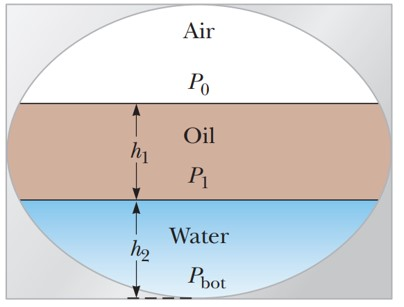
\includegraphics[scale=0.4]{../figs/G10-BAI13-4}}
	\loigiai{
		$p_d=p_0+\rho_1gh_1=\SI{1.013E5}{\pascal}+\left(\SI{700}{\kilogram/\meter^3}\right)\cdot\left(\SI{10}{\meter/\second^2}\right)\cdot\left(\SI{8}{\meter}\right)=\SI{157.3}{\kilo\pascal}$;\\
		$p_n=p_d+\rho_2gh_2=\SI{157.3}{\kilo\pascal}+\left(\SI{1025}{\kilogram/\meter^3}\right)\cdot\left(\SI{10}{\meter/\second^2}\right)\cdot\left(\SI{5}{\meter}\right)=\SI{208.55}{\kilo\pascal}$.
	}
\end{ex}
% ======================================================================
\begin{ex}
	\immini{Hình bên là hệ thống thủy lực để nâng ô tô trong các garage. Khí nén tác dụng lực $F_1$ lên piston nhỏ, hình tròn có bán kính $r_1=\SI{5.00}{\centi\meter}$. Áp suất này được truyền đi nguyên vẹn bởi chất lỏng lí tưởng (chất lỏng không nén) tới piston thứ hai có bán kính $r_2=\SI{15.00}{\centi\meter}$.\begin{enumerate}[label=\alph*)]
			\item Lực tác dụng của khí nén phải có độ lớn bao nhiêu để nâng một ô tô có trọng lượng $\SI{13300}{\newton}$?
			\item Tính áp suất của khí nén.
			\item Để nâng xe lên độ cao $\SI{1}{\meter}$ thì piston thứ nhất phải hạ xuống một đoạn bao nhiêu?
	\end{enumerate}}
	{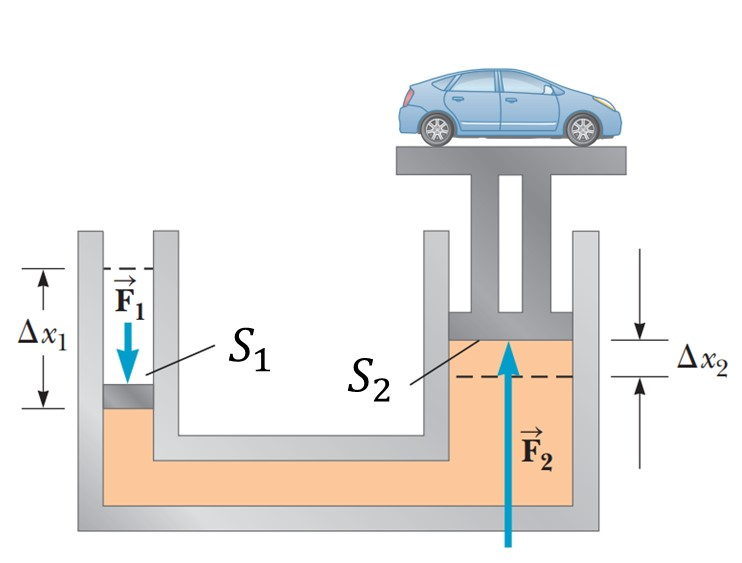
\includegraphics[scale=0.5]{../figs/G10-BAI13-6}}
	
	\loigiai{\begin{enumerate}[label=\alph*)]
			\item $\dfrac{F_1}{S_1}=\dfrac{F_2}{S_2}\Rightarrow F_1=F_2\cdot\dfrac{r^2_2}{r^2_1}=\dfrac{F_1}{9}=\SI{1.48e3}{\newton}$.
			\item $p_1=\dfrac{F_1}{\pi r^2_1}=\SI{1.88E5}{\pascal}$.
			\item $S_1\Delta x_1=S_2\Delta x_2\Rightarrow \Delta x_1=9\Delta x_2=\SI{9}{\meter}$.
	\end{enumerate}}
\end{ex}
\begin{center}
	\textbf{ -- HẾT TIẾT 1 --}
\end{center}